\documentclass{article}

\usepackage[left=1.5in, right=1.5in, top=1in, bottom=1in]{geometry}

\usepackage{tikz}
\usepackage{lscape}
\usepackage{graphicx}
\usepackage{amsmath}
\usepackage{amssymb}
\usepackage{hyperref}
\usepackage{array}

\usepackage{graphicx}
\graphicspath{ {./img/} }

\usepackage[backend=biber]{biblatex}
\bibliography{sources.bib}

\title{Comparing Models of Delta-Notch Signalling}  
\author{Riley Wheadon, Edwin Huras, Ziyi Zhuang}

\begin{document}

\maketitle

\begin{flushleft}

\section*{Abstract}

The Delta-Notch signalling pathway plays a crucial role in determining the cell fate of initially homogeneous cells in a wide array biological systems.
Early deterministic models of the Delta-Notch pathway achieved cell differentiation in linear and 2D cell arrays using highly simplified equations that abstracted away the biochemistry of the system.
In this paper, we present a simple yet biologically realistic model of Delta-Notch signalling and test it using three modelling formalisms: deterministic ODE, stochastic ODE, and agent-based.
Using the Kolmogorov forward equations, we show that the agent-based formalisms converges to the system of deterministic ODEs in expectation.
We also demonstrate that the stochastic ODE and agent-based formalisms can produce cell differentiation even from identical initial conditions.
Finally, we study the effect of parameters such as stochastic noise, domain size, and boundary conditions on the behaviour of our models.
Our findings provide important insights into how different mathematical formalisms can affect simulations of the Delta-Notch signalling network with significant implications for future modelling work. 

\section*{Introduction}

Cell differentiation is essential for the creation of structure in all complex organisms.
Surprisingly, only a small number of signalling pathways are responsible for this essential functions \cite{bray_notch_2006}.
One of these pathways is the Delta-Notch signalling network, which is unique because its ligands Delta and Jagged are transmembrane proteins.
This means that Delta-Notch signalling is largely restricted to neighbouring cells. 
However, new findings suggest that cellular protrusions can allow a small fraction of Delta-Notch signals to travel longer distances \cite{berkemeier_coupling_2023}.
The Delta-Notch signalling network has been shown to affect neurogenesis in vertebrates by determining which cells adopt neural or glial fates. 
Furthermore, mutations in Notch activity has been shown to be a contributing factor to many cancers \cite{bray_notch_2006}.

\medskip

% TODO: Insert a figure here. The paragraph below should be a caption.

\medskip

Binding of the Delta ligand from cell $B$ to the Notch receptor on cell $A$ results in the \emph{cleavage} (removal) of both the ligand and receptor \cite{bray_notch_2006}.
This interaction triggers the release of NICD (Notch Intracellular Domain) in cell $A$, which \emph{promotes} Notch and \emph{inhibits} Delta.
It is also possible for a Delta ligand to bind to a Notch receptor on the same cell. This phenomenon, known as \emph{cis-inhibition}, cleaves the Notch receptor but does not release NICD.
Serrate (Jagged) is a ligand similar to Delta which can also bind to Notch.
However, NICD promotes Serrate, which creates a double-positive feedaback loop.

\medskip

Previous models of Delta-Notch signalling \cite{collier_pattern_1996, boareto_jaggeddelta_2015} have made a number of assumptions which we also use for our models.
First, cells interact through Delta-Notch signalling if and only if they are adjacent.
Production of Notch is an increasing hill function of Delta in neighbouring cells.
Production of Delta is a decreasing hill function of Notch in the same cell.
Both Notch and Delta decay at a rate proportional to their concentration.
Low levels of Notch cause the primary fate, high levels cause the secondary fate.
The behaviour   of cells with a specific fate depends on the specifics of the organism and organ, which is outside the scope of these models. 

\medskip

The model of Delta-Notch signalling proposed by Collier et al. \cite{collier_pattern_1996} makes other simplifications which violate our current understanding of the Notch signalling pathways.
These simplifications make it difficult to identify how individual chemical reactions are captured by the model.
For instance, production of activated Notch (NICD) is exclusively a function of the Delta concentration in neighbouring cells, with no regard for the concentration of Notch receptors.
This violates the mass-balance equations, since the quantity of Notch receptors changes dynamically in response to the concentration of Delta ligands in nearby cells.
There are smaller issues, like the absence of cis-inhibition and the Serrate (Jagged)
protein, but these aren’t necessary to capture the fundamental behaviour of the
system.

\medskip

In this paper, we develop three models of the Delta-Notch signalling network based on a modern understanding of the biochemistry of the system. 
Our first model is an agent-based simulation of individual Delta and Notch molecules. 
While this model is more accurate to the biology than an ODE model, it is impossible to analyze analytically and slow to test numerically.
Then, we define two ODE models. 
The deterministic ODE model defines the behaviour of the agent-based model in expectation (see the Appendix for a proof).
The stochastic ODE model is an extension to the deterministic ODE model which contains noise terms that are intended to simulate the randomness of the agent-based model.
We compare these models with each other using a combination of analytical and numerical methods in a variety of different domains and boundary conditions.
Furthermore, we show that our models qualitatively replicate the results of Collier et al. \cite{collier_pattern_1996}. 
In particular we show that a if linear array of cells is given no-flux boundary conditions, the pattern of alternating cell fates arises on the outside edges before gradually spreading inwards towards the center of the domain.
Additionally, both our model and the Collier et al. model exhibit different ratios of primary to secondary fated cells depending on the parameters on a two-dimensional hexagonal lattice. 

\section*{Methods}

From the literature \cite{collier_pattern_1996, boareto_jaggeddelta_2015}, we assume Notch ($N$) receptor production has the form $H^{+}(I) = n_{m}I^2/(n_{0}^2 + I^2)$ where $I$ is the NICD concentration and $n_{m}, n_{0}$ are hill function parameters.
Similarly, Delta ligand ($D$) production is governed by a decreasing hill function of the for production has the form $H^{-}(I) = d_{m}d_{0}^2/(d_{0}^2 + I^2)$.
Furthermore, we will asume that Notch and Delta both have decay rate $\gamma$.
The variable $k_{T}$ will denote the binding rate between Notch receptors and Delta ligands.
$\gamma_{I}$ is the decay rate of NICD.
We will also assume that there is no cis-interaction and no Serrate ligand. 

\begin{table}[!htp]
\centering
\begin{tabular}{|m{8em}|m{5em}|m{20em}|} 
 \hline
 Reaction & Rate & Description \\ 
 \hline
 $N_{A} + D_{B} \rightarrow I_{A}$ & 
 $k_{T} N_{A}D_{B}$ &
 A Notch receptor from cell $A$ binds to a delta ligand from cell $B$, triggering the release of NICD in cell $A$. \\
 \hline
 $N_{A} \rightarrow \emptyset$ & 
 $\gamma N_{A}$ & 
 A Notch receptor from cell $A$ decays. \\
 \hline
 $D_{A} \rightarrow \emptyset$ & 
 $\gamma D_{A}$ & 
 A Delta receptor from cell $A$ decays. \\
 \hline
 $I_{A} \rightarrow \emptyset$ &
 $\gamma_{I} I_{A}$ &
 A NICD molecule from cell $A$ decays.  \\
 \hline
 $\emptyset \rightarrow N_{A}$ & 
 $H^{+}(I_{A})$ &
 A Notch receptor in cell $A$ is produced \\
 \hline
 $\emptyset \rightarrow D_{A}$ &
 $H^{-}(I_{A})$ &
 A Delta ligand in cell $A$ is produced \\
 \hline
\end{tabular}
\caption{
  A list of possible reactions and their rates in a cell $A$ with neighbour $B$.
  Since there are $6$ possible reactions per cell, a system with $n$ cells will have $6n$ possible reactions to keep track of.
}
\label{tb:reactions}
\end{table}

\medskip

We will make the assumption that reaction times follow a Poisson point process.
Let $E$ be the set of all possible reaction events (i.e. the $6$ reactions above for all cells).
Furthermore, let $|E| = N$ be the number of possible reactions.
For each event, let $X_{i} \sim \text{Exp}(\lambda_{i})$ denote the time until the next event of type $i$, where $1 \leq i \leq N$.
Then, the waiting time $T$ in between \emph{any} two events is:

$$
T = \text{min} \{ X_{1}, \dots, X_{N} \} \sim \text{Exp}\left( \sum_{i = 1}^{N} \lambda_{i} \right) 
$$

This results follows from the definition of an exponential distribution and the memoryless property.
Then, we can use Gillespie's algorithm to simulate the system.
This is the \emph{agent-based} model.
Details of the computational implementation of this model can be found in Appendix \ref{sec:gillespie}.

\medskip

In expectation, the agent-based model converges to the system of ODEs shown in Equation \ref{eq:deterministic}.
A proof of this fact can be found in the appendix.
This is the \emph{deterministic ODE} model, which is described below for a single cell in a two-cell system.
However, this model can be extended to arbitrary domains by defining equations $dN_{i}/dt$, $dD_{i}/dt$, and $dI_{i}/dt$ for each $i \in \{ 1, \dots, n \}$, where $n$ is the number of cells.
In a domain of arbitrary size, $N_{ext}$ and $D_{ext}$ denote the average Notch and Delta concentration over all neighbours.

\begin{equation}
\begin{aligned}
  \frac{dN}{dt} &= \frac{n_{m}I^2}{n_{0}^2 + I^2} - k_{T}ND_{ext} - \gamma N \\[5pt]
  \frac{dD}{dt} &= \frac{d_{m}d_{0}^2}{d_{0}^2 + I^2} - k_{T}DN_{ext} - \gamma D \\[5pt]
  \frac{dI}{dt} &= k_{T}ND_{ext} - \gamma_{I}I
\end{aligned}
\label{eq:deterministic}
\end{equation}

This model is a simplification of Boareto et al. \cite{boareto_jaggeddelta_2015}, which included an additonal equation for the Jagged molecule and kept track of cis-inhibition.
To more directly compare our results with those of Collier et al. \cite{collier_pattern_1996}, we ignore Jagged interactions and cis-inhibition.
Adding NICD, which was absent from Collier et al., was necessary for the assignment of probabilities to each reaction event.
An analysis of the system of ODEs in Equation \ref{eq:deterministic} for fixed values of $N_{ext}, D_{ext}$ reveals an $N = 0$ steady state (the \emph{primary fate}) for all parameter values.
There is also a high Notch steady state (the \emph{secondary fate}) which emerges from a fold bifurcation when $D_{ext}$ is sufficiently large.
See Appendix \ref{sec:bifurcation} for more information.

\medskip

To capture the inherent randomness in receptor-ligand interactions while maintaining computational efficiency, we implement a \emph{stochastic ODE} model based on the chemical Langevin equation formalism.
This approach represents an intermediate level of detail between the deterministic ODE model and the fully discrete Gillespie algorithm.
Starting from the deterministic ODE model described in Equation \ref{eq:deterministic}, we incorporate stochastic fluctuations by adding noise terms proportional to the square root of the reaction rates to get Equation \ref{eq:stochastic}.

\begin{equation}
\begin{aligned}
  dN &= \left( \frac{n_{m}I^2}{n_{0}^2 + I^2} - k_{T}ND_{ext} - \gamma N \right) dt + \sigma \cdot N \cdot dW_{N} \\[5pt]
  dD &= \left( \frac{d_{m}d_{0}^2}{d_{0}^2 + I^2} - k_{T}DN_{ext} - \gamma D \right)  dt + \sigma \cdot D \cdot dW_{D}  \\[5pt]
  dI &= \left( k_{T}ND_{ext} - \gamma_{I}I \right) dt + \sigma \cdot I \cdot dW_{I}
\end{aligned}
\label{eq:stochastic}
\end{equation}

where $dW_N$, $dW_D$, and $dW_I$ are independent Wiener processes representing white noise.
The structure of the noise terms follows from the assumption that noise in each reaction channel is proportional to the current concentration of those molecules.

\medskip

To implement these models computationally, we employed the Euler-Maruyama scheme with time step $dt$.
The deterministic step is first calculated, and then the Wiener increments are sampled from a normal distribution with mean 0 and standard deviation $\sqrt{dt}$.
Each increment is scaled by the its respective variable and added to the results of the deterministic step.

\section*{Results}

% TODO: Write some filler text to connect the different experiments.

\begin{figure}
  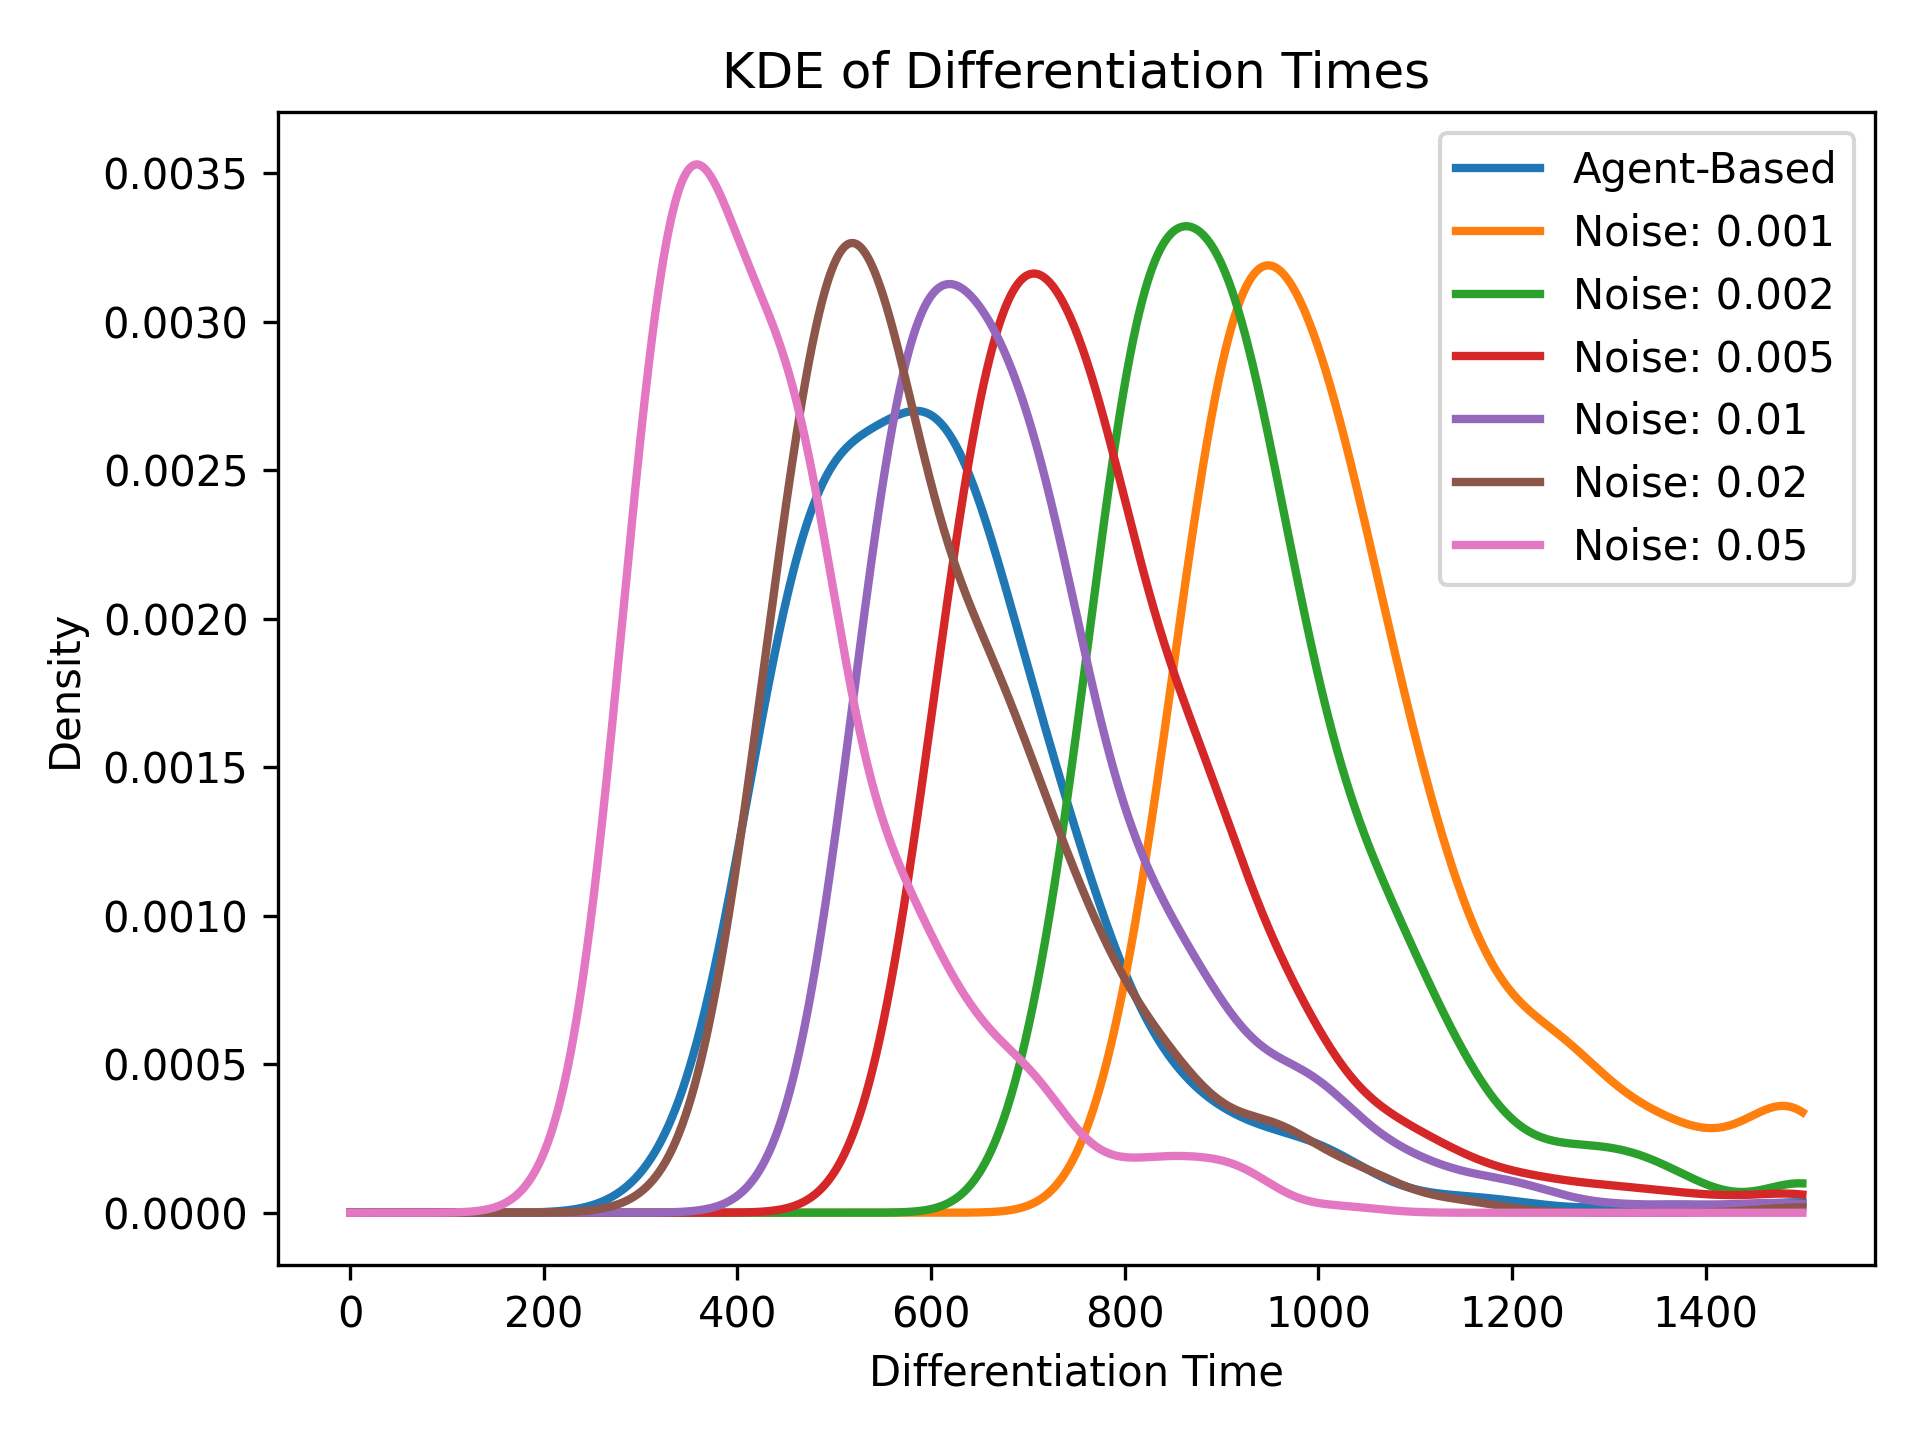
\includegraphics[width=\textwidth]{img/vis11.png}
  \caption{A plot of the KDE approximation of the distribution of differentiation times for the agent-based model and the stochastic ODE model with different levels of noise. All simulations were done on a two-cell domain with periodic boundary conditions. These simulations show that higher values of the noise parameter significantly decrease the average time it takes for the two cells to adopt different fates. Notably, a noise parameter of $2\%$ causes the stochastic ODE model to align most closely with the results of agent-based simulations. }
\end{figure}

\begin{figure}
  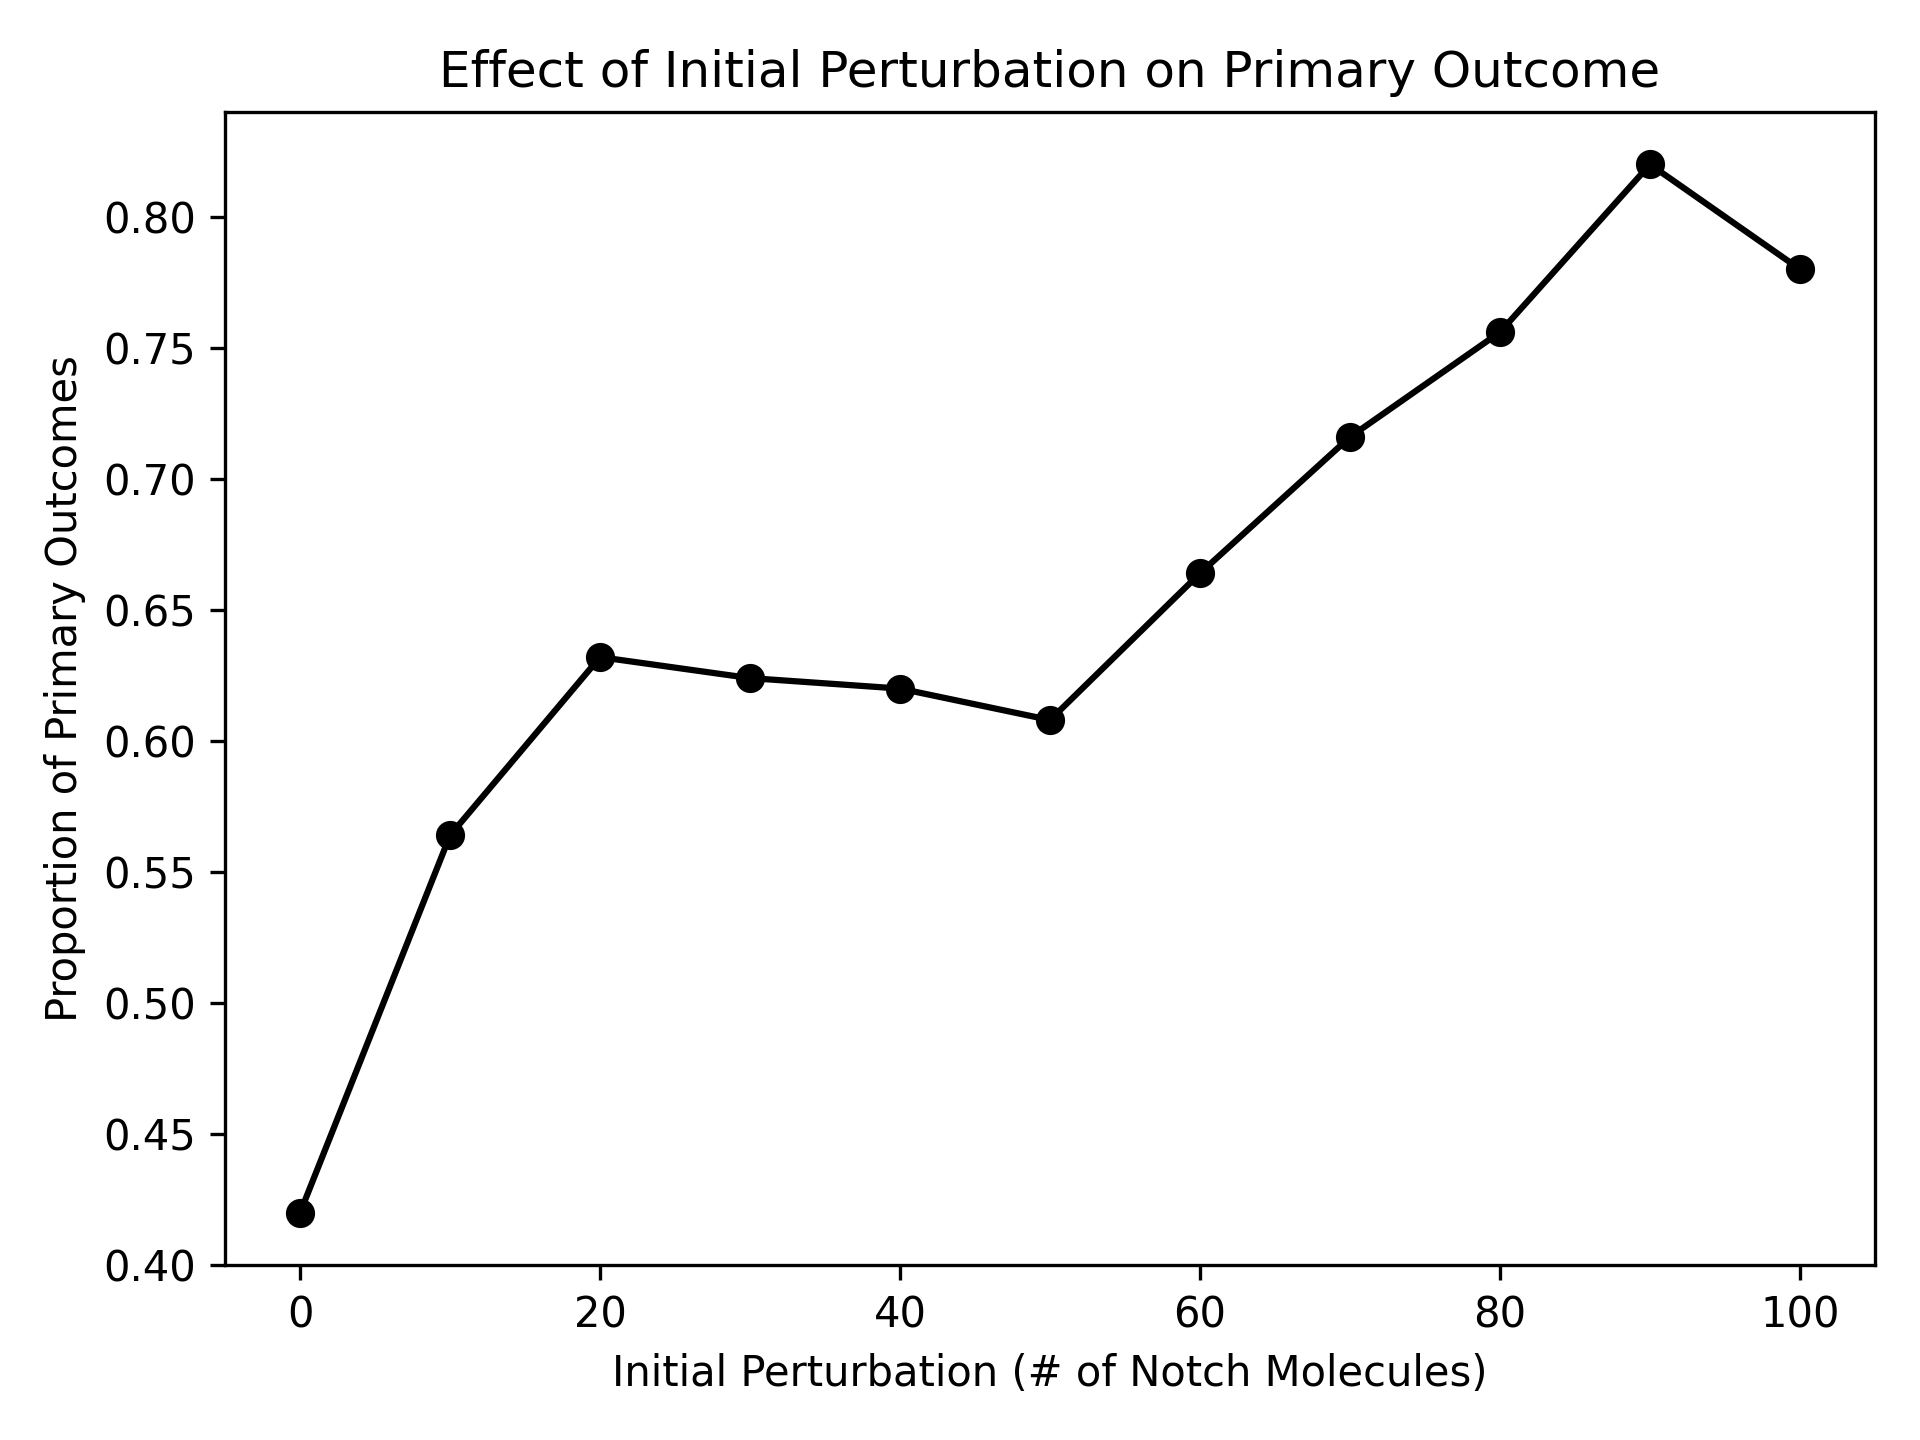
\includegraphics[width=\textwidth]{img/vis12.png}
  \caption{A \emph{Primary Outcome} occurs when the cell with the lower initial Notch concentration ends up adopting the primary (low Notch) fate. This plot shows the relationship between initial perturbation and the sample proportion of primary outcomes for the agent-based model on a two-cell domain. Prior to the perturbation, each cell has $200$ Notch molecules. A perturbation of $x$ molecules removes $x/2$ Notch molecules from the first cell and adds $x/2$ Notch molecules to the second. Unsurprisingly, larger initial perturbations result in a higher proportion of primary outcomes, although this effect is not as extreme as we expected. Even in the largest perturbation we tested ($\pm 25\%$), only $80\%$ of the simulations had the primary outcome. This suggests that it is difficult to reliably control cell fate by perturbation alone.}
\end{figure}

\begin{figure}[!ht]
   \makebox[\textwidth][c]{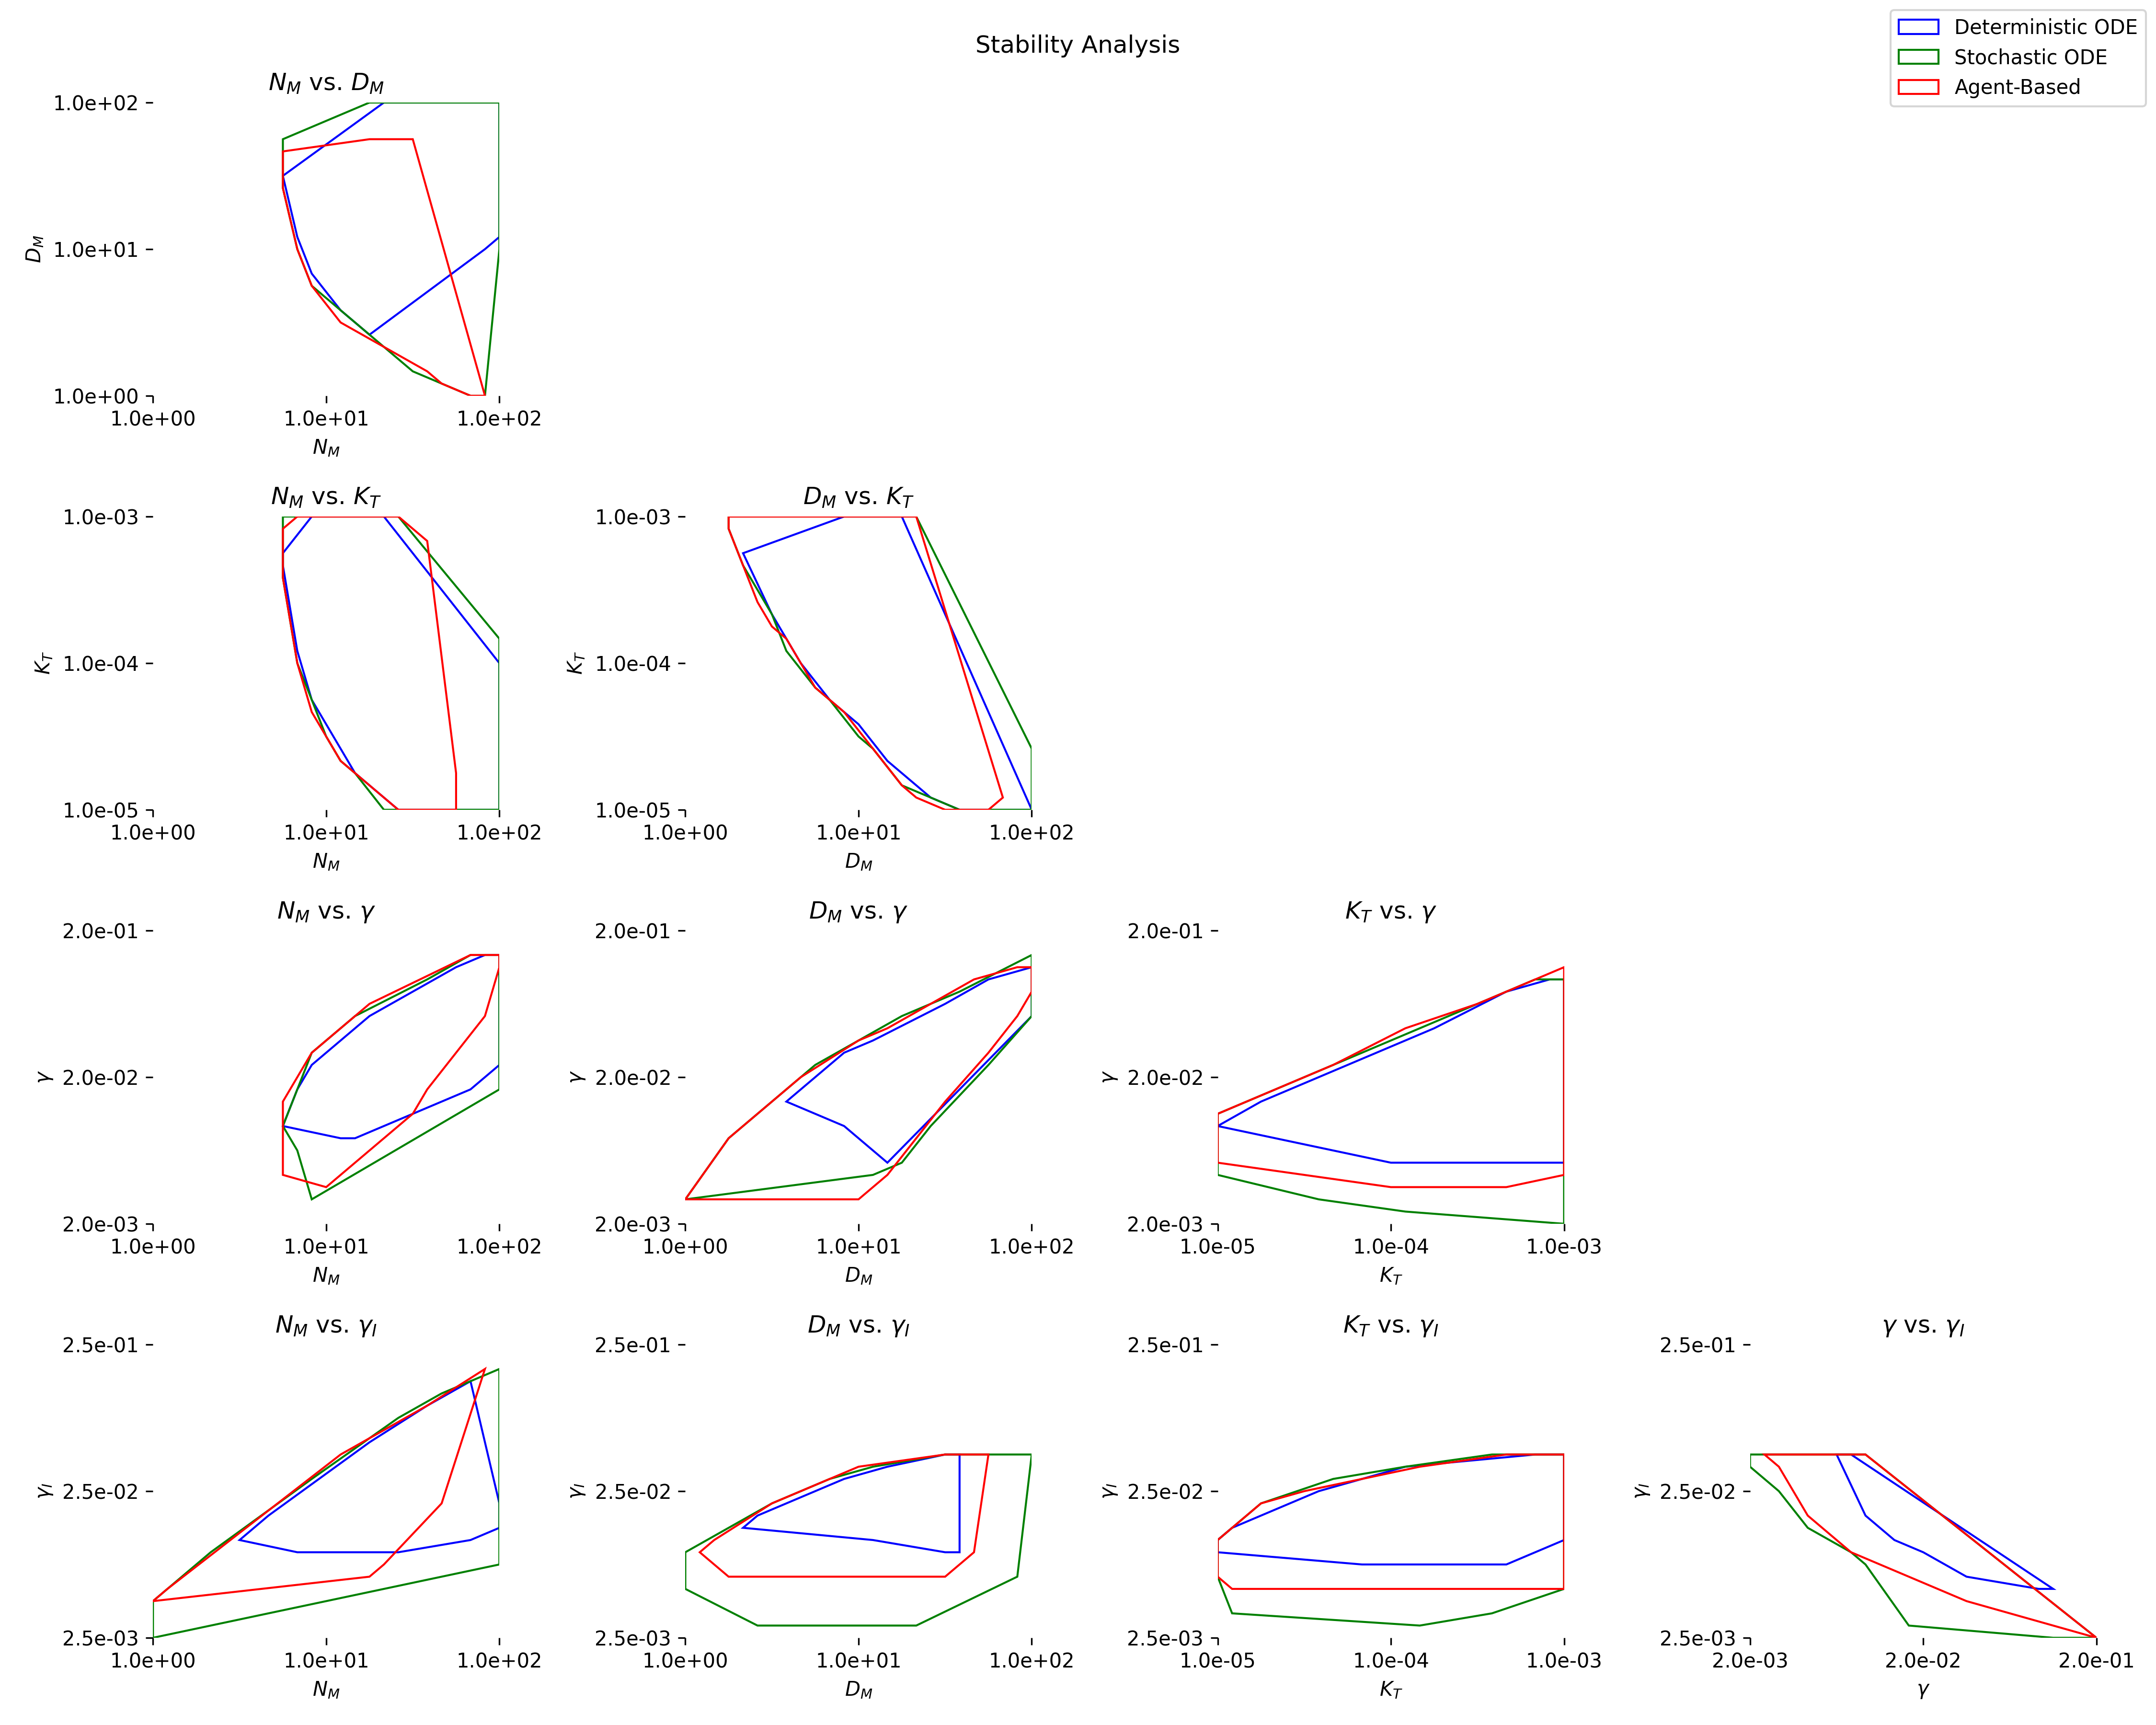
\includegraphics[width=1.3\textwidth]{img/vis13.png}}
   \caption{Results of two-at-a-time stability analysis of the deterministic, stochastic, and agent-based modelling formalisms on a two-cell domain with periodic boundary conditions. The regions enclosed by the red, blue, and green lines are regions in which cell differentiation occurs for each of the three models. Regions were obtained by simulating a $25 \times 25$ grid of test points and taking the convex hull of the points at which cell differentiation occurred. This analysis suggests that the deterministic and stochastic ODE models are on average less sensitive to changes in parameter values than the agent-based model. In particular, the agent-based model does not achieve cell differentiation for large values of the Notch and Delta production parameters $n_{m}$ and $d_{m}$.} 
\end{figure}

\begin{table}[!htp]
\centering
\begin{tabular}{|c|c|c|c|} 
 \hline
 Pattern & Frequency (Odd Domain) & Frequency (Even Domain)  \\
 \hline
 $0: [], \, 1: []$ & $87$ & $403$ \\
 $0: [], \, 1: [2]$ & $801$ & $123$ \\
 $0: [], \, 1: [2, 2]$ & $27$ & $424$ \\
 $0: [], \, 1: [2, 2, 2]$ & $48$ & $1$ \\
 \hline
\end{tabular}
\caption{
  Frequency of selected cell patterns in $1000$ simulations of the agent-based model on $9$-cell (even) and $10$-cell (odd) domains with zero-flux boundary conditions. A \emph{pattern} describes the contiguous groups of cells which share a fate. The pattern $0: [], \, 1: []$ means that cells have alternating fates. The pattern $0: [], \, 1: [2, 2]$ means there are two adjacent pairs of cells with the secondary fate $1$. We observe significant variations in patterns accross even and odd domains. Similarly drastic variation is observed accross different modelling formalisms and boundary conditions (not shown).
}
\label{tb:patterns}
\end{table}

% TODO: Add results on hexagonal domains.

\section*{Discussion}

% TODO: Write this section. Should only need 2-3 paragraphs.

\nocite{*}
\printbibliography

\appendix

\section{Gillespie's Algorithm} \label{sec:gillespie}

Gillespie's algorithm allows us to simulate many types reactions simultaneously using random time steps. Recall that $T_{i}$ is a random variable that represents the distribution of the next reaction of any type. The random variables $X_{1}, \dots, X_{N}$ are the waiting time distributions for each reaction $1, \dots, N$, where $N = (6 \times \text{\# Cells})$.

\medskip

\textbf{Step 1}: Sample a value $t_{i}$ from $T$ using inverse transform sampling. 

\medskip

\textbf{Step 2}: Increment the current time $t$ by $t_{i}$.

\medskip

\textbf{Step 3}: Determine which event took place. To do this, recall that:

$$P(X_{k} = \text{min} \{  X_{1}, \dots, X_{N} \}) = \frac{\lambda_{k}}{\lambda_{1} + \dots + \lambda_{N}}$$

Use this fact to partition the interval $[0, 1]$. Then sample $y_{i}$ from a $\text{Unif}(0, 1)$ distribution, identify its partition, and find the corresponding event.

\medskip

\textbf{Step 4}: Update the state based on the event determined in the previous step.

\medskip

\textbf{Remark}: The expected time for reaction $i$ to occur is given by $\mathbb{E}[X_{i}] = 1/\lambda_{i}$. Therefore, the rate at which event $i$ occurs is $\lambda_{i}$, which is equal to the rate at which the event occurs in the original ODE. This means that the trajectories generated from the Gillespie's algorithm implementation of the agent-based  model can be compared directly to the trajectories generated from the ODE itself, without any need for scaling.

\section{Kolmogorov Forward Equations}
\label{sec:kfe}

% TODO: Revise this section to incorporate Eric's feedback.

\subsection*{Derivation of Kolmogorov Forward Equation}

Let us define $P(n,d,i,t)$ to be the probability of having $n$ Notch receptors, $d$ Delta ligands, and $i$ NICD molecules at time $t$. The Kolmogorov forward equation describes how $P(n,d,i,t)$ changes over a small time step $\Delta t$:

\begin{align*}
P(n,d,i,t+\Delta t) &= P(n,d,i,t) \\
&+ P(n-1,d,i,t) \cdot H^+(i) \Delta t \quad \text{(Notch production)} \\
&+ P(n,d-1,i,t) \cdot H^-(i) \Delta t \quad \text{(Delta production)} \\
&+ P(n+1,d,i,t) \cdot \gamma(n+1)\Delta t \quad \text{(Notch decay)} \\
&+ P(n,d+1,i,t) \cdot \gamma(d+1)\Delta t \quad \text{(Delta decay)} \\
&+ P(n,d,i+1,t) \cdot \gamma_I(i+1)\Delta t \quad \text{(NICD decay)} \\
&+ P(n+1,d,i-1,t) \cdot k_T(n+1)D_{ext}\Delta t \quad \text{(Trans-activation)} \\
&- P(n,d,i,t) \cdot [H^+(i) + H^-(i) + \gamma n + \gamma d + \gamma_I i + k_T n D_{ext}]\Delta t
\end{align*}

Rearranging to find the time derivative:

\begin{align*}
\frac{P(n,d,i,t+\Delta t) - P(n,d,i,t)}{\Delta t} &= P(n-1,d,i,t) \cdot H^+(i) \\
&+ P(n,d-1,i,t) \cdot H^-(i) \\
&+ P(n+1,d,i,t) \cdot \gamma(n+1) \\
&+ P(n,d+1,i,t) \cdot \gamma(d+1) \\
&+ P(n,d,i+1,t) \cdot \gamma_I(i+1) \\
&+ P(n+1,d,i-1,t) \cdot k_T(n+1)D_{ext} \\
&- P(n,d,i,t) \cdot [H^+(i) + H^-(i) + \gamma n + \gamma d + \gamma_I i + k_T n D_{ext}]
\end{align*}

Taking the limit as $\Delta t \rightarrow 0$:

\begin{align*}
\frac{\partial P(n,d,i,t)}{\partial t} &= P(n-1,d,i,t) \cdot H^+(i) \\
&+ P(n,d-1,i,t) \cdot H^-(i) \\
&+ P(n+1,d,i,t) \cdot \gamma(n+1) \\
&+ P(n,d+1,i,t) \cdot \gamma(d+1) \\
&+ P(n,d,i+1,t) \cdot \gamma_I(i+1) \\
&+ P(n+1,d,i-1,t) \cdot k_T(n+1)D_{ext} \\
&- P(n,d,i,t) \cdot [H^+(i) + H^-(i) + \gamma n + \gamma d + \gamma_I i + k_T n D_{ext}]
\end{align*}

\subsection*{Matrix Formulation}
The Kolmogorov forward equation can be expressed in matrix form as:
\[
\frac{d\vec{P}(t)}{dt} = \mathbf{A} \vec{P}(t)
\]

where $\vec{P}(t)$ is a column vector containing the probabilities for all possible states, and $\mathbf{A}$ is the transition rate matrix. \\

To construct the matrix $\mathbf{A}$, we first establish a one-to-one mapping between the three-dimensional state space $(n,d,i)$ and a one-dimensional index $k$. For a system with maximum values $n_{max}$, $d_{max}$, and $i_{max}$, we define:
\[
k(n,d,i) = n \cdot (d_{max}+1) \cdot (i_{max}+1) + d \cdot (i_{max}+1) + i
\]
for $0 \leq n \leq n_{max}, \; 0 \leq d \leq d_{max}, \; 0 \leq i \leq i_{max}$.

The inverse mapping gives:
\begin{align*}
n(k) &= \left\lfloor \frac{k}{(d_{max}+1) \cdot (i_{max}+1)} \right\rfloor \\
d(k) &= \left\lfloor \frac{k \bmod ((d_{max}+1) \cdot (i_{max}+1))}{i_{max}+1} \right\rfloor \\
i(k) &= k \bmod (i_{max}+1)
\end{align*}

With this mapping, we can now define the elements of matrix $\mathbf{A}$. Let $k$ and $k'$ be the indices corresponding to states $(n,d,i)$ and $(n',d',i')$ respectively:

\begin{align*}
A_{k',k} = 
\begin{cases}
H^+(i) & \text{if } (n',d',i') = (n+1,d,i) \quad \text{(Notch production)} \\
H^-(i) & \text{if } (n',d',i') = (n,d+1,i) \quad \text{(Delta production)} \\
\gamma(n) & \text{if } (n',d',i') = (n-1,d,i) \quad \text{(Notch decay)} \\
\gamma(d) & \text{if } (n',d',i') = (n,d-1,i) \quad \text{(Delta decay)} \\
\gamma_I(i) & \text{if } (n',d',i') = (n,d,i-1) \quad \text{(NICD decay)} \\
k_T(n)D_{ext} & \text{if } (n',d',i') = (n-1,d,i+1) \quad \text{(Trans-activation)} \\
-\sum_{k'' \neq k} A_{k'',k} & \text{if } k' = k \quad \text{(Diagonal terms)}
\end{cases}
\end{align*}

Note that $A_{k',k}$ represents the transition rate from state $k$ to state $k'$. The diagonal elements $A_{k,k}$ are the negative sum of all outgoing rates from state $k$:

\[
A_{k,k} = -[H^+(i) + H^-(i) + \gamma n + \gamma d + \gamma_I i + k_T n D_{ext} + k_T d N_{ext}]
\]

where $(n,d,i)$ is the state corresponding to index $k$.\\

The resulting matrix $\mathbf{A}$ is a sparse matrix with the following properties:
\begin{itemize}
    \item Dimension: $(n_{max}+1) \cdot (d_{max}+1) \cdot (i_{max}+1) \times (n_{max}+1) \cdot (d_{max}+1) \cdot (i_{max}+1)$
    \item Number of non-zero elements: $\approx 7 \cdot (n_{max}+1) \cdot (d_{max}+1) \cdot (i_{max}+1)$
\end{itemize}

To illustrate, let's consider a minimal system with $n_{max} = d_{max} = i_{max} = 1$. This gives us 8 possible states:
$(0,0,0)$, $(0,0,1)$, $(0,1,0)$, $(0,1,1)$, $(1,0,0)$, $(1,0,1)$, $(1,1,0)$, $(1,1,1)$

The corresponding transition matrix $\mathbf{A}$ would be:

\begin{align*}
\mathbf{A} = 
\begin{pmatrix}
-\alpha_{000} & \gamma_I & \gamma & 0 & \gamma & 0 & 0 & 0 \\
H^+(0) & -\alpha_{001} & 0 & \gamma & 0 & \gamma & 0 & 0 \\
H^-(0) & 0 & -\alpha_{010} & \gamma_I & 0 & 0 & \gamma & 0 \\
0 & H^-(0) & H^+(0) & -\alpha_{011} & 0 & 0 & 0 & \gamma \\
H^+(0) & 0 & 0 & 0 & -\alpha_{100} & \gamma_I & \gamma & 0 \\
0 & H^+(0) & 0 & 0 & H^+(1) & -\alpha_{101} & 0 & \gamma \\
0 & 0 & H^+(0) & 0 & H^-(1) & 0 & -\alpha_{110} & \gamma_I \\
0 & 0 & 0 & H^+(0) & 0 & H^-(1) & H^+(1) & -\alpha_{111}
\end{pmatrix}
\end{align*}

where:
\[
\alpha_{ndi} = H^+(i) + H^-(i) + \gamma n + \gamma d + \gamma_I i + k_T n D_{ext} + k_T d N_{ext}
\]

Additionally, we need to add the terms for trans-activation, which would connect states like $(1,0,0)$ to $(0,0,1)$ with rate $k_T \cdot 1 \cdot D_{ext}$.\\

For a fully labelled matrix with all transitions explicitly shown, the matrix for $n_{max} = d_{max} = i_{max} = 1$ would be:

\[
\mathbf{A} = 
\begin{bmatrix}
A_{11} & A_{12} & A_{13} & A_{14} & A_{15} & A_{16} & A_{17} & A_{18} \\
B_{11} & B_{12} & B_{13} & B_{14} & B_{15} & B_{16} & B_{17} & B_{18} \\
C_{11} & C_{12} & C_{13} & C_{14} & C_{15} & C_{16} & C_{17} & C_{18} \\
D_{11} & D_{12} & D_{13} & D_{14} & D_{15} & D_{16} & D_{17} & D_{18} \\
E_{11} & E_{12} & E_{13} & E_{14} & E_{15} & E_{16} & E_{17} & E_{18} \\
F_{11} & F_{12} & F_{13} & F_{14} & F_{15} & F_{16} & F_{17} & F_{18} \\
G_{11} & G_{12} & G_{13} & G_{14} & G_{15} & G_{16} & G_{17} & G_{18} \\
H_{11} & H_{12} & H_{13} & H_{14} & H_{15} & H_{16} & H_{17} & H_{18}
\end{bmatrix}
\]

where  

\begin{tiny}
\begin{align*}
A_{11} &= -(H^+(0) + H^-(0)),  & A_{12} &= \gamma_I,  \\
A_{13} &= \gamma,  & A_{14} &= 0,  \\
A_{15} &= \gamma,  & A_{16} &= 0,  \\
A_{17} &= 0,  & A_{18} &= 0,  \\[5pt]
B_{11} &= H^+(0),  & B_{12} &= -(H^+(1) + H^-(1) + \gamma_I),  \\
B_{13} &= 0,  & B_{14} &= \gamma,  \\
B_{15} &= k_T D_{ext},  & B_{16} &= \gamma,  \\
B_{17} &= 0,  & B_{18} &= 0,  \\[5pt]
C_{11} &= H^-(0),  & C_{12} &= 0,  \\
C_{13} &= -(H^+(0) + H^-(0) + \gamma + k_T N_{ext}),  & C_{14} &= \gamma_I,  \\
C_{15} &= 0,  & C_{16} &= 0,  \\
C_{17} &= \gamma,  & C_{18} &= 0,  \\[5pt]
D_{11} &= 0,  & D_{12} &= H^-(1),  \\
D_{13} &= H^+(0),  & D_{14} &= -(H^+(1) + H^-(1) + \gamma + \gamma_I + k_T N_{ext}),  \\
D_{15} &= 0,  & D_{16} &= k_T D_{ext},  \\
D_{17} &= 0,  & D_{18} &= \gamma,  \\[5pt]
E_{11} &= H^+(0),  & E_{12} &= 0,  \\
E_{13} &= 0,  & E_{14} &= 0,  \\
E_{15} &= -(H^+(0) + H^-(0) + \gamma + k_T D_{ext}),  & E_{16} &= \gamma_I,  \\
E_{17} &= \gamma,  & E_{18} &= 0,  \\[5pt]
F_{11} &= 0,  & F_{12} &= H^+(1),  \\
F_{13} &= 0,  & F_{14} &= 0,  \\
F_{15} &= H^+(0),  & F_{16} &= -(H^+(1) + H^-(1) + \gamma + \gamma_I + k_T D_{ext}),  \\
F_{17} &= 0,  & F_{18} &= \gamma,  \\[5pt]
G_{11} &= 0,  & G_{12} &= 0,  \\
G_{13} &= H^+(0),  & G_{14} &= 0,  \\
G_{15} &= H^-(0),  & G_{16} &= 0,  \\
G_{17} &= -(H^+(0) + H^-(0) + \gamma + \gamma + k_T D_{ext} + k_T N_{ext}),  & G_{18} &= \gamma_I,  \\[5pt]
H_{11} &= 0,  & H_{12} &= 0,  \\
H_{13} &= 0,  & H_{14} &= H^+(1),  \\
H_{15} &= 0,  & H_{16} &= H^-(1),  \\
H_{17} &= H^+(0),  & H_{18} &= -(H^+(1) + H^-(1) + \gamma + \gamma + \gamma_I + k_T D_{ext} + k_T N_{ext}).
\end{align*}
\end{tiny}

Each row and column corresponds to a state in the order:
$(0,0,0)$, $(0,0,1)$, $(0,1,0)$, $(0,1,1)$, $(1,0,0)$, $(1,0,1)$, $(1,1,0)$, $(1,1,1)$

The matrix element $A_{j,i}$ represents the transition rate from state $i$ to state $j$. The diagonal elements $A_{i,i}$ contain the negative sum of all outgoing rates from state $i$.


\section{Theoretical Justification}
\label{sec:theoretical-justification}

% TODO: Revise this section to incorporate Eric's feedback.

In this section, we need to show that in expectation, the model above converges to the following system of ODEs (adapted from Boareto et al., 2015):

$$
\begin{aligned}
  \frac{dN}{dt} &= \frac{n_{m}I^2}{n_{0}^2 + I^2} - k_{T}ND_{ext} - \gamma N \\[5pt]
  \frac{dD}{dt} &= \frac{d_{m}d_{0}^2}{d_{0}^2 + I^2} - k_{T}DN_{ext} - \gamma D \\[5pt]
  \frac{dI}{dt} &= k_{T}ND_{ext} - \gamma_{I}I
\end{aligned}
$$

\subsection*{Setup and Notation}

Let us define:
\begin{itemize}
  \item $\langle N \rangle = \sum_{n,d,i} n \cdot P(n,d,i,t)$ = expected number of Notch receptors
  \item $\langle D \rangle = \sum_{n,d,i} d \cdot P(n,d,i,t)$ = expected number of Delta ligands
  \item $\langle I \rangle = \sum_{n,d,i} i \cdot P(n,d,i,t)$ = expected number of NICD molecules
\end{itemize}

\subsection*{Deriving ODEs for Expected Values}

\textbf{Now we derive the ODE for the expected value of Notch:}

\begin{align*}
\frac{d\langle N \rangle}{dt} &= \frac{d}{dt}\sum_{n,d,i} n \cdot P(n,d,i,t) \\
&= \sum_{n,d,i} n \cdot \frac{\partial P(n,d,i,t)}{\partial t}
\end{align*}

Substituting the Kolmogorov forward equation:

\begin{align*}
\frac{d\langle N \rangle}{dt} &= \sum_{n,d,i} n \cdot \Big[ P(n-1,d,i,t) \cdot H^+(i) \\
&+ P(n,d-1,i,t) \cdot H^-(i) \\
&+ P(n+1,d,i,t) \cdot \gamma(n+1) \\
&+ P(n,d+1,i,t) \cdot \gamma(d+1) \\
&+ P(n,d,i+1,t) \cdot \gamma_I(i+1) \\
&+ P(n+1,d,i-1,t) \cdot k_T(n+1)D_{ext} \\
&- P(n,d,i,t) \cdot [H^+(i) + H^-(i) + \gamma n + \gamma d + \gamma_I i + k_T n D_{ext}] \Big]
\end{align*}

Now we use index shifting to simplify.\\~\\

\textbf{(A) Notch Production} \\
Let's substitute $n' = n-1$ (so $n = n'+1$):
\begin{align*}
\sum_{n,d,i} n \cdot P(n-1,d,i,t) \cdot H^+(i) &= \sum_{n',d,i} (n'+1) \cdot P(n',d,i,t) \cdot H^+(i) \\
&= \sum_{n',d,i} n' \cdot P(n',d,i,t) \cdot H^+(i) + \sum_{n',d,i} P(n',d,i,t) \cdot H^+(i) \\
&= \sum_{n,d,i} n \cdot P(n,d,i,t) \cdot H^+(i) + \sum_{n,d,i} P(n,d,i,t) \cdot H^+(i) \\
\end{align*}

The first term is $\langle N \cdot H^+(I) \rangle$. If we assume that $H^+(I)$ is approximately $H^+(\langle I \rangle)$, then this term becomes $\langle N \rangle \cdot H^+(\langle I \rangle)$. The second term is $\langle H^+(I) \rangle \approx H^+(\langle I \rangle)$. 

So the contribution of this term is:
\[
\sum_{n,d,i} n \cdot P(n-1,d,i,t) \cdot H^+(i) \approx \langle N \rangle \cdot H^+(\langle I \rangle) + H^+(\langle I \rangle)
\]

Since we are indexing from 0, and $n-1$ could be negative, the sum should start from $n=1$:

\begin{small}
\begin{align*}
\sum_{n \geq 1,d,i} n \cdot P(n-1,d,i,t) \cdot H^+(i) &= \sum_{n' \geq 0,d,i} (n'+1) \cdot P(n',d,i,t) \cdot H^+(i) \\
&= \sum_{n' \geq 0,d,i} n' \cdot P(n',d,i,t) \cdot H^+(i) + \sum_{n' \geq 0,d,i} P(n',d,i,t) \cdot H^+(i) \\
&= \langle N \rangle \cdot H^+(\langle I \rangle) + H^+(\langle I \rangle) \\
&= H^+(\langle I \rangle) \cdot (1 + \langle N \rangle)
\end{align*}
\end{small}

\textbf{(B) Delta Production}\\
This term does not affect $N$, so the prefactor $n$ remains with the original probability:
\begin{align*}
\sum_{n,d,i} n \cdot P(n,d-1,i,t) \cdot H^-(i) &= \sum_{n,d',i} n \cdot P(n,d',i,t) \cdot H^-(i) \\
&= \langle N \cdot H^-(I) \rangle \\
&\approx \langle N \rangle \cdot H^-(\langle I \rangle)
\end{align*}

\textbf{(C) Notch Decay}
\begin{align*}
\sum_{n,d,i} n \cdot P(n+1,d,i,t) \cdot \gamma(n+1) &= \sum_{n',d,i} (n'-1) \cdot P(n',d,i,t) \cdot \gamma n' \\
&= \gamma \sum_{n',d,i} (n'-1)n' \cdot P(n',d,i,t) \\
&= \gamma \sum_{n',d,i} n'^2 \cdot P(n',d,i,t) - \gamma \sum_{n',d,i} n' \cdot P(n',d,i,t) \\
&= \gamma(\langle N^2 \rangle - \langle N \rangle)
\end{align*}

If we assume that the variance of $N$ is small compared to its mean (which is reasonable for high molecule counts), then $\langle N^2 \rangle \approx \langle N \rangle^2$. So:
\begin{align*}
\gamma(\langle N^2 \rangle - \langle N \rangle) &\approx \gamma(\langle N \rangle^2 - \langle N \rangle) \\
&= \gamma \langle N \rangle (\langle N \rangle - 1)
\end{align*}

\textbf{(D) Delta Decay}
\begin{align*}
\sum_{n,d,i} n \cdot P(n,d+1,i,t) \cdot \gamma(d+1) &= \gamma \sum_{n,d',i} n \cdot P(n,d',i,t) \cdot d' \\
&= \gamma \langle N \cdot D \rangle \\
&\approx \gamma \langle N \rangle \langle D \rangle
\end{align*}

\textbf{(E) NICD Decay}
\begin{align*}
\sum_{n,d,i} n \cdot P(n,d,i+1,t) \cdot \gamma_I(i+1) &= \gamma_I \sum_{n,d,i'} n \cdot P(n,d,i',t) \cdot i' \\
&= \gamma_I \langle N \cdot I \rangle \\
&\approx \gamma_I \langle N \rangle \langle I \rangle
\end{align*}

\textbf{(F) Trans-activation}
\begin{align*}
\sum_{n,d,i} n \cdot P(n+1,d,i-1,t) \cdot k_T(n+1)D_{ext} &= k_T D_{ext} \sum_{n',d,i'} (n'-1) \cdot P(n',d,i',t) \cdot n' \\
&= k_T D_{ext} \sum_{n',d,i'} (n'^2 - n') \cdot P(n',d,i',t) \\
&= k_T D_{ext} (\langle N^2 \rangle - \langle N \rangle) \\
&\approx k_T D_{ext} \langle N \rangle (\langle N \rangle - 1)
\end{align*}

\textbf{(G) Negative Terms}
\begin{align*}
&-\sum_{n,d,i} n \cdot P(n,d,i,t) \cdot [H^+(i) + H^-(i) + \gamma n + \gamma d + \gamma_I i + k_T n D_{ext}] \\
&= -\langle N \cdot H^+(I) \rangle - \langle N \cdot H^-(I) \rangle - \gamma \langle N^2 \rangle - \gamma \langle N \cdot D \rangle - \gamma_I \langle N \cdot I \rangle - k_T D_{ext} \langle N^2 \rangle \\
&\approx -\langle N \rangle \cdot H^+(\langle I \rangle) - \langle N \rangle \cdot H^-(\langle I \rangle) - \gamma \langle N \rangle^2 - \gamma \langle N \rangle \langle D \rangle - \gamma_I \langle N \rangle
\langle I \rangle - k_T D_{ext} \langle N \rangle^2
\end{align*} \\~\\

\textbf{(H) Final Synthesis of $\langle N \rangle$}\\

Combining all these terms:

\begin{align*}
\frac{d\langle N \rangle}{dt} &= H^+(\langle I \rangle) \cdot (1 + \langle N \rangle) + \langle N \rangle \cdot H^-(\langle I \rangle) + \gamma \langle N \rangle (\langle N \rangle - 1) + \gamma \langle N \rangle \langle D \rangle \\
&+ \gamma_I \langle N \rangle \langle I \rangle + k_T D_{ext} \langle N \rangle (\langle N \rangle - 1) \\
&- \langle N \rangle \cdot H^+(\langle I \rangle) - \langle N \rangle \cdot H^-(\langle I \rangle) - \gamma \langle N \rangle^2 - \gamma \langle N \rangle \langle D \rangle - \gamma_I \langle N \rangle \langle I \rangle - k_T D_{ext} \langle N \rangle^2 \\
\end{align*}

After cancellations:

\begin{align*}
\frac{d\langle N \rangle}{dt} &= H^+(\langle I \rangle) + \langle N \rangle \cdot H^+(\langle I \rangle) + \gamma \langle N \rangle (\langle N \rangle - 1) + k_T D_{ext} \langle N \rangle (\langle N \rangle - 1) \\
&- \langle N \rangle \cdot H^+(\langle I \rangle) - \gamma \langle N \rangle^2 - k_T D_{ext} \langle N \rangle^2 \\
&= H^+(\langle I \rangle) + \gamma \langle N \rangle (\langle N \rangle - 1) - \gamma \langle N \rangle^2 + k_T D_{ext} \langle N \rangle (\langle N \rangle - 1) - k_T D_{ext} \langle N \rangle^2 \\
&= H^+(\langle I \rangle) + \gamma \langle N \rangle (\langle N \rangle - 1 - \langle N \rangle) + k_T D_{ext} \langle N \rangle (\langle N \rangle - 1 - \langle N \rangle) \\
&= H^+(\langle I \rangle) - \gamma \langle N \rangle - k_T D_{ext} \langle N \rangle \\
\end{align*}

Therefore, the ODE for $\langle N \rangle$ is:

\[
\frac{d\langle N \rangle}{dt} = H^+(\langle I \rangle) - \gamma \langle N \rangle - k_T D_{ext} \langle N \rangle
\]

Substituting the definition of $H^+(\langle I \rangle)$:

\[
\frac{d\langle N \rangle}{dt} = \frac{n_m \langle I \rangle^2}{n_0^2 + \langle I \rangle^2} - \gamma \langle N \rangle - k_T D_{ext} \langle N \rangle
\]

Which can be written as:

\[
\frac{dN}{dt} = \frac{n_m I^2}{n_0^2 + I^2} - \gamma N - k_T D_{ext} N
\]

where we use $N$, $D$, and $I$ as shorthand for the expected values $\langle N \rangle$, $\langle D \rangle$, and $\langle I \rangle$.\\~\\

\textbf{Similarly, we can derive the ODE for the expected value of Delta:}

\begin{align*}
\frac{d\langle D \rangle}{dt} &= \frac{d}{dt}\sum_{n,d,i} d \cdot P(n,d,i,t) \\
&= \sum_{n,d,i} d \cdot \frac{\partial P(n,d,i,t)}{\partial t}
\end{align*}

We will analyse each term of the Kolmogorov equation, multiplied by $d$, as follows.

\[
\sum_{n,d,i} d \cdot P(n-1,d,i,t) \cdot H^+(i) = \langle D \cdot H^+(I) \rangle \approx \langle D \rangle \cdot H^+(\langle I \rangle)
\]

\[
\sum_{n,d,i} d \cdot P(n,d-1,i,t) \cdot H^-(i) = \langle D \cdot H^-(I) \rangle + \langle H^-(I) \rangle 
\approx \langle D \rangle \cdot H^-(\langle I \rangle) + H^-(\langle I \rangle)
\]

\[
\sum_{n,d,i} d \cdot P(n+1,d,i,t) \cdot \gamma(n+1) \approx \gamma \langle D \rangle \langle N \rangle
\]

\[
\sum_{n,d,i} d \cdot P(n,d+1,i,t) \cdot \gamma(d+1) \approx \gamma \langle D \rangle (\langle D \rangle - 1)
\]

\[
\sum_{n,d,i} d \cdot P(n,d,i+1,t) \cdot \gamma_I(i+1) \approx \gamma_I \langle D \rangle \langle I \rangle
\]

\[
\sum_{n,d,i} d \cdot P(n+1,d,i-1,t) \cdot k_T(n+1)D_{ext} \approx k_T D_{ext} \langle D \rangle \langle N \rangle
\]

Now we consider this term which appears in the ODEs but was not explicitly stated in our Kolmogorov equation setup. This is a special case where we need to account for Delta from our cell binding to Notch in neighbouring cells:

\begin{align*}
-\sum_{n,d,i} d \cdot P(n,d,i,t) \cdot k_T d N_{ext} &= -k_T N_{ext} \sum_{n,d,i} d^2 \cdot P(n,d,i,t) \\
&= -k_T N_{ext} \langle D^2 \rangle \\
&\approx -k_T N_{ext} \langle D \rangle^2
\end{align*}

Now we consider negative terms from original equation.
\begin{align*}
&-\sum_{n,d,i} d \cdot P(n,d,i,t) \cdot [H^+(i) + H^-(i) + \gamma n + \gamma d + \gamma_I i + k_T n D_{ext}] \\
&\approx -\langle D \rangle \cdot H^+(\langle I \rangle) - \langle D \rangle \cdot H^-(\langle I \rangle) - \gamma \langle D \rangle \langle N \rangle - \gamma \langle D \rangle^2 - \gamma_I \langle D \rangle \langle I \rangle - k_T D_{ext} \langle D \rangle \langle N \rangle
\end{align*}

Let's synthesise all terms of $\langle D \rangle$

\begin{align*}
\frac{d\langle D \rangle}{dt} &= \langle D \rangle \cdot H^+(\langle I \rangle) + \langle D \rangle \cdot H^-(\langle I \rangle) + H^-(\langle I \rangle) + \gamma \langle D \rangle \langle N \rangle \\
&+ \gamma \langle D \rangle (\langle D \rangle - 1) + \gamma_I \langle D \rangle \langle I \rangle + k_T D_{ext} \langle D \rangle \langle N \rangle - k_T N_{ext} \langle D \rangle^2 \\
&- \langle D \rangle \cdot H^+(\langle I \rangle) - \langle D \rangle \cdot H^-(\langle I \rangle) - \gamma \langle D \rangle \langle N \rangle - \gamma \langle D \rangle^2 - \gamma_I \langle D \rangle \langle I \rangle - k_T D_{ext} \langle D \rangle \langle N \rangle \\
&= H^-(\langle I \rangle) - \gamma \langle D \rangle - k_T N_{ext} \langle D \rangle^2
\end{align*}

Making a final approximation that $\langle D \rangle^2 \approx \langle D \rangle$, we get:

\[
\frac{d\langle D \rangle}{dt} = H^-(\langle I \rangle) - \gamma \langle D \rangle - k_T N_{ext} \langle D \rangle
\]

Substituting the definition of $H^-(\langle I \rangle)$:

\[
\frac{d\langle D \rangle}{dt} = \frac{d_m}{d_0^2 + \langle I \rangle^2} - \gamma \langle D \rangle - k_T N_{ext} \langle D \rangle
\]

Which can be written as:

\[
\frac{dD}{dt} = \frac{d_m}{d_0^2 + I^2} - \gamma D - k_T N_{ext} D
\]

\textbf{Finally, we derive the ODE for NICD:}

\begin{align*}
\frac{d\langle I \rangle}{dt} &= \frac{d}{dt}\sum_{n,d,i} i \cdot P(n,d,i,t) \\
&= \sum_{n,d,i} i \cdot \frac{\partial P(n,d,i,t)}{\partial t}
\end{align*}

Let's analyse each term:

\[
\sum_{n,d,i} i \cdot P(n-1,d,i,t) \cdot H^+(i) = \langle I \cdot H^+(I) \rangle \approx \langle I \rangle \cdot H^+(\langle I \rangle)
\]

\[
\sum_{n,d,i} i \cdot P(n,d-1,i,t) \cdot H^-(i) \approx \langle I \rangle \cdot H^-(\langle I \rangle)
\]

\[
\sum_{n,d,i} i \cdot P(n+1,d,i,t) \cdot \gamma(n+1) \approx \gamma \langle I \rangle \langle N \rangle
\]

\[
\sum_{n,d,i} i \cdot P(n,d+1,i,t) \cdot \gamma(d+1) \approx \gamma \langle I \rangle \langle D \rangle
\]

\[
\sum_{n,d,i} i \cdot P(n,d,i+1,t) \cdot \gamma_I(i+1) \approx \gamma_I \langle I \rangle (\langle I \rangle - 1)
\]

\[
\sum_{n,d,i} i \cdot P(n+1,d,i-1,t) \cdot k_T(n+1)D_{ext} \approx k_T D_{ext} \langle I \rangle \langle N \rangle + k_T D_{ext} \langle N \rangle
\]

Negative terms can be rewritten as:
\begin{align*}
&-\sum_{n,d,i} i \cdot P(n,d,i,t) \cdot [H^+(i) + H^-(i) + \gamma n + \gamma d + \gamma_I i + k_T n D_{ext}] \\
&\approx -\langle I \rangle \cdot H^+(\langle I \rangle) - \langle I \rangle \cdot H^-(\langle I \rangle) - \gamma \langle I \rangle \langle N \rangle - \gamma \langle I \rangle \langle D \rangle - \gamma_I \langle I \rangle^2 - k_T D_{ext} \langle I \rangle \langle N \rangle
\end{align*}

Let's combine all terms for $\langle I \rangle$

\begin{align*}
\frac{d\langle I \rangle}{dt} &= \langle I \rangle \cdot H^+(\langle I \rangle) + \langle I \rangle \cdot H^-(\langle I \rangle) + \gamma \langle I \rangle \langle N \rangle + \gamma \langle I \rangle \langle D \rangle \\
&+ \gamma_I \langle I \rangle (\langle I \rangle - 1) + k_T D_{ext} \langle I \rangle \langle N \rangle + k_T D_{ext} \langle N \rangle \\
&- \langle I \rangle \cdot H^+(\langle I \rangle) - \langle I \rangle \cdot H^-(\langle I \rangle) - \gamma \langle I \rangle \langle N \rangle - \gamma \langle I \rangle \langle D \rangle - \gamma_I \langle I \rangle^2 - k_T D_{ext} \langle I \rangle \langle N \rangle \\
\end{align*}

Therefore, the ODE for $\langle I \rangle$ is:
\[
\frac{d\langle I \rangle}{dt} = k_T D_{ext} \langle N \rangle - \gamma_I \langle I \rangle
\]

Which can be written as:

\[
\frac{dI}{dt} = k_T D_{ext} N - \gamma_I I
\]

\subsection*{Final System of ODEs}

Combining our three derived equations, we get the following system of ODEs:

\begin{align*}
\frac{dN}{dt} &= \frac{n_m I^2}{n_0^2 + I^2} - \gamma N - k_T D_{ext} N \\
\frac{dD}{dt} &= \frac{d_m}{d_0^2 + I^2} - \gamma D - k_T N_{ext} D \\
\frac{dI}{dt} &= k_T D_{ext} N - \gamma_I I
\end{align*}

This matches the system presented in section 3.6 of the document:

\begin{align*}
\frac{dN}{dt} &= \frac{n_m I^2}{n_0^2 + I^2} - k_T N D_{ext} - \gamma N \\
\frac{dD}{dt} &= \frac{d_m}{d_0^2 + I^2} - k_T D N_{ext} - \gamma D \\
\frac{dI}{dt} &= k_T N D_{ext} - \gamma_I I
\end{align*}

\subsection*{Mapping Between Probabilities and Rates}

To relate the probabilistic formulation to the deterministic ODE system, we need to understand how reaction probabilities map to reaction rates. In the stochastic formulation, the probability of a reaction occurring in a small time interval $\Delta t$ is:
\begin{align*}
P(\text{reaction}) \approx \text{rate} \times \Delta t
\end{align*}

For example:

\[
P(\emptyset \rightarrow N_A) = H^+(I) \Delta t = \frac{n_m I^2}{n_0^2 + I^2} \Delta t 
\]

In the limit as $\Delta t \rightarrow 0$, these probabilities per unit time become rates, which appear directly in the deterministic ODEs. The ODE system essentially tracks the expected values of these stochastic processes under the assumption that fluctuations are small compared to the means.

\section{Bifurcation Analysis}
\label{sec:bifurcation}

\subsection*{One-Cell System}

First, we consider the one-cell system under the influence of a second, static cell. In this model, the Notch and Delta concentrations in the second cell ($N_{ext}$ and $D_{ext}$) are treated as parameters. Equations \ref{eq:one-cell-notch}, \ref{eq:one-cell-delta}, and \ref{eq:one-cell-nicd} define this system.

\begin{align}
  \label{eq:one-cell-notch}
  \frac{dN}{dt} &= \frac{n_{m}I^2}{n_{0}^2 + I^2} - (k_{T}D_{ext} + \gamma)N \\[5pt]
  \label{eq:one-cell-delta}
  \frac{dD}{dt} &= \frac{d_{m}d_{0}^2}{d_{0}^2 + I^2} - (k_{T}N_{ext} + \gamma)D \\[5pt]
  \label{eq:one-cell-nicd}
  \frac{dI}{dt} &= k_{T}ND_{ext} - \gamma_{I}I
\end{align}

Observe that $dN/dt$ and $dI/dt$ do not depend on $D$. Therefore, we can analyze the $N-I$ phase plane to learn more about the system. First, we find the nullclines of Equations \ref{eq:one-cell-notch} and \ref{eq:one-cell-nicd} as functions of $I$. The results of this calculation are shown in Equations \ref{eq:one-cell-notch-nullcline} and \ref{eq:one-cell-nicd-nullcline}.

\begin{align}
  \label{eq:one-cell-notch-nullcline}
  f_{N}(I) &= \frac{1}{\gamma + k_{T}D_{ext}}\left(\frac{n_{m}I^2}{n_{0}^2 + I^2}\right) \\[5pt]
  \label{eq:one-cell-nicd-nullcline}
  f_{I}(I) &= \frac{\gamma_{I}I}{k_{T}D_{ext}}
\end{align}

Plotting the nullclines in Equations \ref{eq:one-cell-notch-nullcline} and \ref{eq:one-cell-nicd-nullcline} on the $N-I$ plane for small and large values of $D_{ext}$ (assuming the other parameters are suitably chosen) reveals a fold bifurcation. 

\begin{figure}[!htp]
  \label{fig:one-cell-phase-plane}
  \centering
  \begin{tikzpicture}[scale=1.75]
    \node[draw] at (1.5,2.5) {Low $D_{ext}$};
    \draw[->] (0, 0) -- (3, 0) node[right] {$I$};
    \draw[->] (0, 0) -- (0, 2) node[above] {$N$};
    \draw[domain= 0:2, smooth, variable=\x, blue] 
      plot ({\x}, {\x});
    \draw[domain= 0:3, smooth, variable=\x, red] 
      plot ({\x}, {(2*\x*\x)/(2 + \x*\x)});
    \draw (0, 0) node[circle,fill,scale=0.5] {};
  \end{tikzpicture}
  \begin{tikzpicture}[scale=1.75]
    \node[draw] at (1.5,2.5) {High $D_{ext}$};
    \draw[->] (0, 0) -- (3, 0) node[right] {$I$};
    \draw[->] (0, 0) -- (0, 2) node[above] {$N$};
    \draw[domain= 0:3, smooth, variable=\x, blue] 
      plot ({\x}, {0.45 * \x});
    \draw[domain= 0:3, smooth, variable=\x, red] 
      plot ({\x}, {(1.5*\x*\x)/(2 + \x*\x)});
    \draw (0, 0) node[circle,fill,scale=0.5] {};
    \draw (0.78475, 0.35314) node[circle,draw=black,fill=white,thick,scale=0.5] {};
    \draw (2.54858, 1.14686) node[circle,fill,scale=0.5] {};
  \end{tikzpicture}
  \caption{Approximate $N-I$ phase planes for the one-cell ODE model under the influence of low and high Delta from a static neighbour. The $N$-nullcline is shown in red and the $I$-nullcline is shown in blue. Below a critical value of $D_{ext}$, the system undergoes a fold bifurcation which results in the annihalation of the high Notch steady state. The high Notch steady state is also absent for qualitativley high values of $\gamma_{I}$, low values of $k_{T}$, and low values of $n_{m}$.}
\end{figure}

\subsection*{Two-Cell System}

Now, we will consider the coupled two-cell system in which both cells respond to the Delta-Notch signalling of the other. Let $N_{1}, D_{1}, I_{1}$ and $N_{2}, D_{2}, I_{2}$ denote the Notch, Delta, and NICD concentrations in the first and second cells respectively. Our previous analysis reveals that the $N_{1} = I_{1} = 0$ steady state exists for all values of $D_{2}$. The steady state concentrations $\{ N_{1}^{*}, D_{1}^{*}, I_{1}^{*}, N_{2}^{*}, D_{2}^{*}, I_{2}^{*} \}$ for this case are given in Equation \ref{eq:two-cell-steady-states}.

\begin{equation}
\label{eq:two-cell-steady-states}
\begin{aligned}
  N_{1}^{*} &= 0  &
  N_{2}^{*} &= \frac{1}{\gamma + k_{T}D_{1}^{*}}\left( \frac{n_{m}(I_{2}^{*})^2}{n_{0}^2 + (I_{2}^{*})^2} \right)  \\[5pt]
  D_{1}^{*} &= \frac{d_{m}}{\gamma + k_{T}N_{2}^{*}} &
  D_{2}^{*} &= \frac{1}{\gamma} \left( \frac{d_{m}d_{0}^2}{d_{0}^2 + (I_{2}^{*})^2} \right)  \\[5pt]
  I_{1}^{*} &= 0 &
  I_{2}^{*} &= \frac{k_{T}N_{2}^{*}D_{1}^{*}}{\gamma_{I}}
\end{aligned}
\end{equation}

There is a second steady state occurs when $N_{1}^{*} = N_{2}^{*}$, $D_{1}^{*} = D_{2}^{*}$, and $I_{1}^{*} = I_{2}^{*}$. While it is difficult to analytically determine the steady state concentrations, we can verify that this steady state exists and is unstable using computer simulations.

\end{flushleft}

\end{document}







